\chapter{Metric Spaces}\label{chapter:metric.spaces}%
\chapterSummary{We study various abstract notions of distance.}

\section{Definition}
A \emph{metric space}\define{metric!space} is a set \(X\) of objects (called points) equipped with a \emph{metric}\define{metric} or \emph{distance function}\define{distance!function}  \(d \colon X \times X \to \R{}\), which assigns to each pair \(x, y\) of points of \(X\) a real number \(d(x, y) \ge 0\), the \emph{distance} from \(x\) to \(y\), so that
\begin{enumerate}
\item \(d(x,x) = 0\) for any \(x \in X\) and
\item if \(x \ne y\) then \(d(x, y) > 0\) and
\item (symmetry) \(d(x,y) = d(y,x)\) for any \(x,y \in X\) and
\item (the triangle inequality\define{triangle inequality}) 
\[
d(x,z) \le d(x,y) + d(y,z) 
\]
for any points \(x,y,z \in X\). Roughly: it is never shorter to go from \(x\) to \(z\) via \(y\) than to go ``directly'' from \(x\) to \(z\).
\end{enumerate}
\begin{example}
The real number line \(\R{}\) is a metric space, with metric \(d(x,y)=|x-y|\) for any two real numbers \(x,y \in \R{}\).
\end{example}
\begin{example}
Euclidean space \(\R{n}\) is a metric space, with the \emph{Euclidean}\define{Euclidean metric}\define{metric!Euclidean} metric \(d(x,y)=\left|x-y\right|\) for any two points \(x,y \in \R{n}\).
\end{example}
\begin{example}
If \(X\) is a metric space, with metric \(d_X\), and \(S \subset X\) is any subset, then \(S\) is a metric space with \(d_S(x,y)=d_X(x,y)\), i.e. restricting the metric on \(X\) to points from \(S\), the \emph{induced metric}\define{induced!metric}\define{metric!induced}.
For instance, the sphere in Euclidean space is a metric space, with this restricted metric.
\end{example}
\begin{example}
Euclidean space \(\R{n}\) is \emph{also} a metric space with various other metrics, for example the \emph{taxi-cab metric}\define{taxi-cab metric}\define{metric!taxi-cab}
\[
d(x,y)=\left|x_1-y_1\right|+\left|x_2-y_2\right|+\dots+\left|x_n-y_n\right|.
\]
This measures the distance we travel in a journey from \(x\) to \(y\) along a path made of line segments parallel to the coordinate axes, just as a taxi-cab in Manhattan can only travel along the streets, which run north-south and east-west.
\end{example}
\begin{example}
Euclidean space admits another usual metric: the sup norm metric
\[
d(x,y)=\max{\left|x_1-y_1\right|, \left|x_2-y_2\right|, \dots, \left|x_n-y_n\right|}.
\]
\end{example}
\begin{example}
Take any collection of dots called \emph{vertices}, connected up by paths called \emph{edges}.
\begin{center}
\documentclass[tikz]{standalone}
\colorlet{exampleBackgroundColour}{white}
\begin{document}
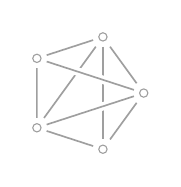
\begin{tikzpicture}[scale=.75]
\foreach \i in {1,...,5}
{%
	\node[gray!75] (vert \i) at ({cos(\i*72)},{sin(\i*72}) {};
	\draw[gray!75] (vert \i) circle (2pt);
}%
\draw[draw=exampleBackgroundColour,very thick,double=gray!75] (vert 1) -- (vert 2) -- (vert 3) -- (vert 4) -- (vert 5) -- (vert 1);
\draw[draw=exampleBackgroundColour,very thick,double=gray!75] (vert 1) -- (vert 4);
\draw[draw=exampleBackgroundColour,very thick,double=gray!75] (vert 1) -- (vert 3);
\draw[draw=exampleBackgroundColour,very thick,double=gray!75] (vert 5) -- (vert 2);
\draw[draw=exampleBackgroundColour,very thick,double=gray!75] (vert 5) -- (vert 3);
\end{tikzpicture}
\end{document}
\end{center}
The resulting drawing is a \emph{graph}.
The graph is \emph{connected} if we can move from any vertex to any other along a sequence of edges.
The \emph{distance} between two vertices is the minimum number of edges we must traverse to travel from one vertex to the other.
\end{example}
\begin{example}
The integrable functions on a measureable set \(A \subset \R{n}\) form a metric space under 
\[
d(f,g)=\int_A |f-g|.
\]
\end{example}
\begin{example}\label{item:product.metrics}
If \(X\) and \(Y\) are metric spaces, then \(X \times Y\) is a metric space with metrics
\[
d_1\of{\pr{x_0,y_0}, \, \pr{x_1,y_1}}
=
d_X\of{x_0,x_1} + d_Y\of{y_0,y_1},
\]
or
\[
d_2\of{\pr{x_0,y_0}, \, \pr{x_1,y_1}}
=
\sqrt{d_X\of{x_0,x_1}^2 + d_Y\of{y_0,y_1}^2},
\]
or
\[
d_3\of{\pr{x_0,y_0}, \, \pr{x_1,y_1}}
=
\max{d_X\of{x_0,x_1},d_Y\of{y_0,y_1}},
\]
among many other possibilities.
\end{example}
\begin{example}
On any set \(X\), the \emph{standard discrete metric}\define{discrete!metric!standard}\define{metric!discrete!standard} is defined by
\[
d(x,y)=
\begin{cases}
0, & \text{ if \(x=y\)}, \\
1, & \text{ if \(x \ne y\)}.
\end{cases}
\]
\end{example}
\begin{example}
The \emph{disjoint union}\define{disjoint union} \(X \sqcup Y\) of two sets \(X\) and \(Y\) is the the set of pairs of the form \((1,x)\) for \(x\) in \(X\) or \((2,y)\) for \(y\) in \(Y\).
In this way, we force each element \(x\) of \(X\) to be represented by a different point \((1,x)\) of \(X \sqcup Y\) than any point of \(Y\).
For example, \(\R{} \sqcup \R{}\) consists of two ``copies'' of the real number line.
Nonetheless, we usual denote the point \((1,x)\) just as \(x\) and the point \((2,y)\) just as \(y\) respectively, if that doesn't cause any confusion.
Given metrics on \(X\) and \(Y\), defined a metric on \(X \sqcup Y\) by \(d(x,y)=1\) for \(x\) in \(X\) and \(y\) in \(Y\), and with points of \(X\) having distances given by the metric on \(X\) and with points of \(Y\) having distances given by the metric on \(Y\).
So \(\R{} \sqcup \R{}\) is a pair of lines, but each point of one line is exactly one unit from each point of the other line: something I can't draw.
\end{example}
\begin{example}
If \(x=\pr{x_1, x_2, \dots}\) and \(y=\pr{y_1, y_2, \dots}\) are two sequences in a metric space \(X\), we can define a distance between sequences as
\[
d(x,y)=\sup_i d_X\of{x_i,y_i}.
\]
The set \(Z\) of all \emph{bounded} sequences in \(X\) is a metric space.
(Unbounded sequences can have infinite distance.)
\end{example}
\begin{problem}{metric.spaces:Hamming}
Suppose that \(A\) is a nonempty set and \(n \ge 1\) is an integer.
Let \(X\defeq A \times A \times \dots \times A=A^n\).
So elements \(x\) of \(X\) look like \(x=(x_1,x_2,\dots,x_n)\) with each of \(x_1,x_2,\dots,x_n\) drawn from \(A\).
The \emph{Hamming distance}\define{Hamming metric} \(d(x,y)\) is
\[
d(x,y)=\#\set{i|x_i\ne y_i}.
\]
Prove that \(d\) is a metric.
\end{problem}
\begin{problem}{metric.spaces:not.in.Kansas}
Give an example of a metric space \(X\) which does not arise as a subspace (with induced metric) of Euclidean space of any dimension.
\end{problem}
\begin{answer}{metric.spaces:not.in.Kansas}
Take a set consisting of 4 points \(X=\set{a,b_0,b_1,c}\).
Set \(d(a,c)=2)\), and all other distances between distinct points set to \(1\).
Then \(d(a,b_i)+d(b_i,c)=d(a,c)\).
So if \(X\) arises as a subspace of \(\R{n}\), then \(b_0\) and \(b_1\) both bisect the line segment \(ac\), so must be equal, so \(X\) has only three points, a contradiction.
This same example applies in any Hilbert space instead of \(\R{n}\).
\end{answer}

\section{Convergence}
A sequence \(x_1, x_2, \dots \in X\) in a metric space \emph{converges}\define{convergence!in a metric space} to a point \(x \in X\), denoted \(x_i \to x\), if the distances \(d\of{x_1,x}, d\of{x_2, x}, \dots\) go to zero.
\begin{problem}{metric.spaces:Hausdorff}
Suppose that a sequence \(x_1, x_2, \dots \in X\) converges to a point \(p \in X\) and also converges to a point \(q \in X\).
Prove that \(p=q\).
\end{problem}
\begin{problem}{metric.spaces:taxi.convergence}
Prove that a sequence in \(\R{n}\) converges in the taxi-cab metric just when it converges in the Euclidean metric.
\end{problem}
\begin{problem}{metric.spaces:discrete:convergence}
When does a sequence converge in a discrete metric?
\end{problem}
\begin{problem}{metric.spaces:discrete:convergence.limit}
Prove that a point \(x \in X\) is an accumulation point of a set \(S \subset X\) just when there is a sequence in \(S\) converging to \(x\).
\end{problem}
A metric is \emph{discrete}\define{metric!discrete}\define{discrete!metric} if any convergent sequence is constant after finitely many steps.
\begin{problem}{metric.spaces:discrete.not.sep}
A metric space is \emph{\(\varepsilon\)-separated} if any distinct points are of distance at least \(\varepsilon\).
Give an example of a discrete metric space which is not \(\varepsilon\)-separated for any \(\varepsilon\).
\end{problem}
\begin{answer}{metric.spaces:discrete.not.sep}
Let \(X\) be the set of points \(1/2, 1/3, \dots \in \R{}\) with induced metric.
\end{answer}

\section{Open and closed sets}
The \emph{ball}\define{ball} (or \emph{open ball}) of radius \(r \ge 0\) about a point \(x \in X\) of a metric space is
\[
\ball[X]{r}{x} = \Set{y \in X|d(x,y)<r},
\]
while the \emph{closed ball} of radius \(r \ge 0\) about a point \(x \in X\) of a metric space is
\[
\ballClosed[X]{r}{x} = \Set{y \in X|d(x,y)\le r}.
\]
\begin{problem}{metric.spaces:balls}
What are the balls of the taxi-cab metric? The sup norm metric? The metric on a graph? 
\end{problem}
An \emph{open set}\define{open!set!in a metric space}\define{set!open!in a metric space} in a metric space \(X\) is a union of open balls.
\begin{problem}{metric.spaces:open.union}
Prove that 
\begin{enumerate}
\item
The empty set is open in any metric space.
\item 
Any metric space is an open subset of itself.
\item
The union of any collection of open sets in a metric space is an open set.
\item
The intersection of any finite collection of open sets in a metric space is an open set.
\end{enumerate}
\end{problem}
\begin{problem}{metric.spaces:discrete.open}
What are the open sets in a discrete metric space?
\end{problem}
A set is \emph{closed}\define{closed!set!in a metric space}\define{set!closed!in a metric space} if its complement is open.
\begin{problem}{metric.spaces:intersect}
Prove that 
\begin{enumerate}
\item
The empty set is closed in any metric space.
\item 
Any metric space is a closed subset of itself.
\item
The intersection of any collection of closed sets in a metric space is a closed set.
\item
The union of any finite collection of closed sets in a metric space is a closed set.
\item
A set consisting of a single point in a metric space is closed.
\end{enumerate}
\end{problem}
\begin{problem}{metric.spaces:discrete.closed}
What are the closed sets in a discrete metric space?
\end{problem}
The \emph{interior}\define{interior} of a set \(S \subset X\) is the union of all open sets lying in \(S\), and hence is itself open.
The \emph{closure}\define{closure!in a metric space} \(\bar{S}\) of a set \(S \subset X\) is the intersection of all closed sets containing it.
\begin{problem}{metric.spaces:limit.points}
An \emph{accumulation point}\define{accumulation point} of a subset \(S \subset X\) of a metric space is a point \(x \in X\) so that every ball containing \(x\) of positive radius intersects \(S\).
Prove that \(\bar{S}\) is the set of accumulation points of \(S\).
\end{problem}
\begin{problem}{metric.spaces:discrete.acc}
What are the accumulation points of a set in a discrete metric space?
\end{problem}
\begin{problem}{metric.spaces:closed.ball}
Give an example of a metric space in which the closure of an open about some point of some radius \(r\) is \emph{not} the closed ball of radius \(r\) about that point.
\end{problem}

\section{Relatively open sets}
A set \(S \subset Y \subset X\) is \emph{relatively open}\define{relatively open}\define{open!relatively} if it is open as a subset of \(Y\) in the induced metric, and we similarly define \emph{relatively closed} subsets of subsets.
\begin{lemma}
A set \(S \subset Y \subset X\) is relatively open just when \(S=Y \cap U\) for some open subset \(U \subset X\).
A set \(S \subset Y \subset X\) is relatively closed just when \(S=Y \cap C\) for some closed subset \(C \subset X\).
\end{lemma}
\begin{proof}
The balls of \(X\) intersect \(Y\) in the balls of \(Y\); picture each ball of \(Y\) extending out to a ball in \(X\).
The open sets of \(Y\) are unions of those balls of \(Y\); just extend each ball.
The proof for closed sets follows easily as they are complements of open sets.
\end{proof}

\section{Completeness}
A \emph{Cauchy sequence} in a metric space \(X\) is a sequence \(x_1, x_2, \dots \in X\) so that the distances \(d\of{x_i,x_j}\) get, and stay, as small as we like, if we go far enough down the sequence, i.e. if \(i\) and \(j\) are both large enough.
\begin{problem}{metric.spaces:conv.Cauchy}
Prove that every convergent sequence is Cauchy.
\end{problem}
A metric space is \emph{complete}\define{complete!metric space}\define{metric!space!complete} if every Cauchy sequence is convergent.
\begin{problem}{metric.spaces:Euclid.complete}
Prove that Euclidean space is complete.
\end{problem}
\begin{example}
The rational numbers form an incomplete metric space, in the induced metric from the real number line, because we can make a sequence of rational approximations to any irrational number, so a Cauchy sequence of rational numbers which does not converge \emph{inside} the space of rational numbers.
\end{example}
\begin{example}
The integrable functions on a measurable set \(A \subset \R{n}\) form a complete metric space, as proven in analysis textbooks.
\end{example}
\begin{problem}{metric.spaces:closed.Cauchy}
Prove that a subset \(S\) of a complete metric space \(X\) is complete in the induced metric just when it is a closed subset of \(X\).
\end{problem}
\begin{problem}{metric.spaces:taxi.complete}
Prove that \(\R{n}\) is complete in the taxi-cab metric.
\end{problem}

\section{Compactness}
A metric space is \emph{compact}\define{compact!metric space}\define{metric!space!compact} if every infinite sequence of points of the metric space has a convergent subsequence.
A subset of a metric space is \emph{compact} if it is a compact metric space in the induced metric.
For example, the empty set is compact in any metric space.
\begin{problem}{metric.spaces:finite.cpt}
Prove that any finite set of points in any metric space is compact.
\end{problem}
\begin{problem}{metric.spaces:finite.cpt.2}
Prove that a finite union of compact sets is compact, and that the intersection of any collection of compact sets is compact.
\end{problem}
A metric space (or subset of a metric space) is bounded if it lies in a ball.
The \emph{diameter}\define{diameter!metric space} is the supremum of distances between points of the metric space, and is finite just when the space is bounded.
An \emph{open cover}\define{open!cover!metric space} of a set in a metric space is a collection of open sets whose union contains the set.
A \emph{subcover}\define{subcover!metric space} of an open cover is a collection of open sets from the cover, which still manage to cover the set.

\begin{theorem}\label{theorem:HB.naive}
A metric space is compact just when every open cover of the metric space has a finite subcover.
Every compact metric space is complete.
\end{theorem}
\begin{proof}
Suppose that every open cover has a finite subcover.
Take a sequence \(x_1, x_2, \dots\) of points in our metric space.
We need to prove there is a convergent subsequence.
We only need prove that some point \(x\) has infinitely many elements of our sequence arbitrarily close to it.
Suppose not.
Then for each point \(x\), we can find an open set \(U_x\) containing \(x\) and only containing finitely many points of our sequence.
Take a finite subcover.
Then there are only finitely many points in our sequence, so it contains a constant subsequence.

Suppose that our metric space is compact.
First, we prove that it is complete.
Every Cauchy sequence \(x_1,x_2,\dots\) has a convergent subsequence, say with a limit \(x\).
Along the subsequence, the points get and stay close to \(x\).
But along the whole sequence, the points stay close to one another, since it is Cauchy.
Therefore the sequence converges.

Next, we prove that, for any \(\varepsilon > 0\), \(X\) is covered by finitely many balls of radius \(\varepsilon\).
(See the next section for more about this property, called \emph{total boundedness}.)
Suppose not.
Then we take any point \(x_1\), and let \(x_2\) be a point of distance at least \(\varepsilon\) from \(x_1\), and \(x_3\)  point of distance at least \(\varepsilon\) from both of \(x_1, x_2\), and so on.
There is no convergent subsequence, a contradiction.

Take an open cover, and let's look for a finite subcover.
Pick a radius \(\varepsilon>0\) and cover by finitely many balls of radius \(\varepsilon\).
If we can cover each of these balls by finitely many open sets from our open cover, then we throw these together to get a finite cover.
So one of our balls admits no finite subcover by our open sets.
Let \(x_1\) be the center of that ball.
Repeat by induction for smaller values of \(\varepsilon\) at each step, to produce a collection of points \(x_1, x_2, \dots\) so that \(d\of{x_j,x_{j+1}}<\varepsilon_j\), with \(\varepsilon_1, \varepsilon_2, \dots \to 0\).
So the ball centers form an infinite sequence; replace by a subsequence to ensure convergence to some point \(x\).
Take an open set from our open cover containing \(x\).
All but finitely many of our points \(x_1, x_2, \dots\) lie in that open set, and so do the balls of radii \(\varepsilon_i\) about them.
But that one open set from our open cover is already a finite subcover of that \(\varepsilon_i\)-ball, a contradiction.
\end{proof}
\begin{problem}{metric.spaces:compact.discrete}
Which discrete metric spaces are compact?
Which are bounded?
\end{problem}

\section{Totally bounded spaces}
Try to approximate a metric space by a discrete metric space: a \emph{\(\varepsilon\)-net}\define{net} is a set of points in a metric space so that every point lies within distance \(\varepsilon\) from a point of that set.
\begin{center}
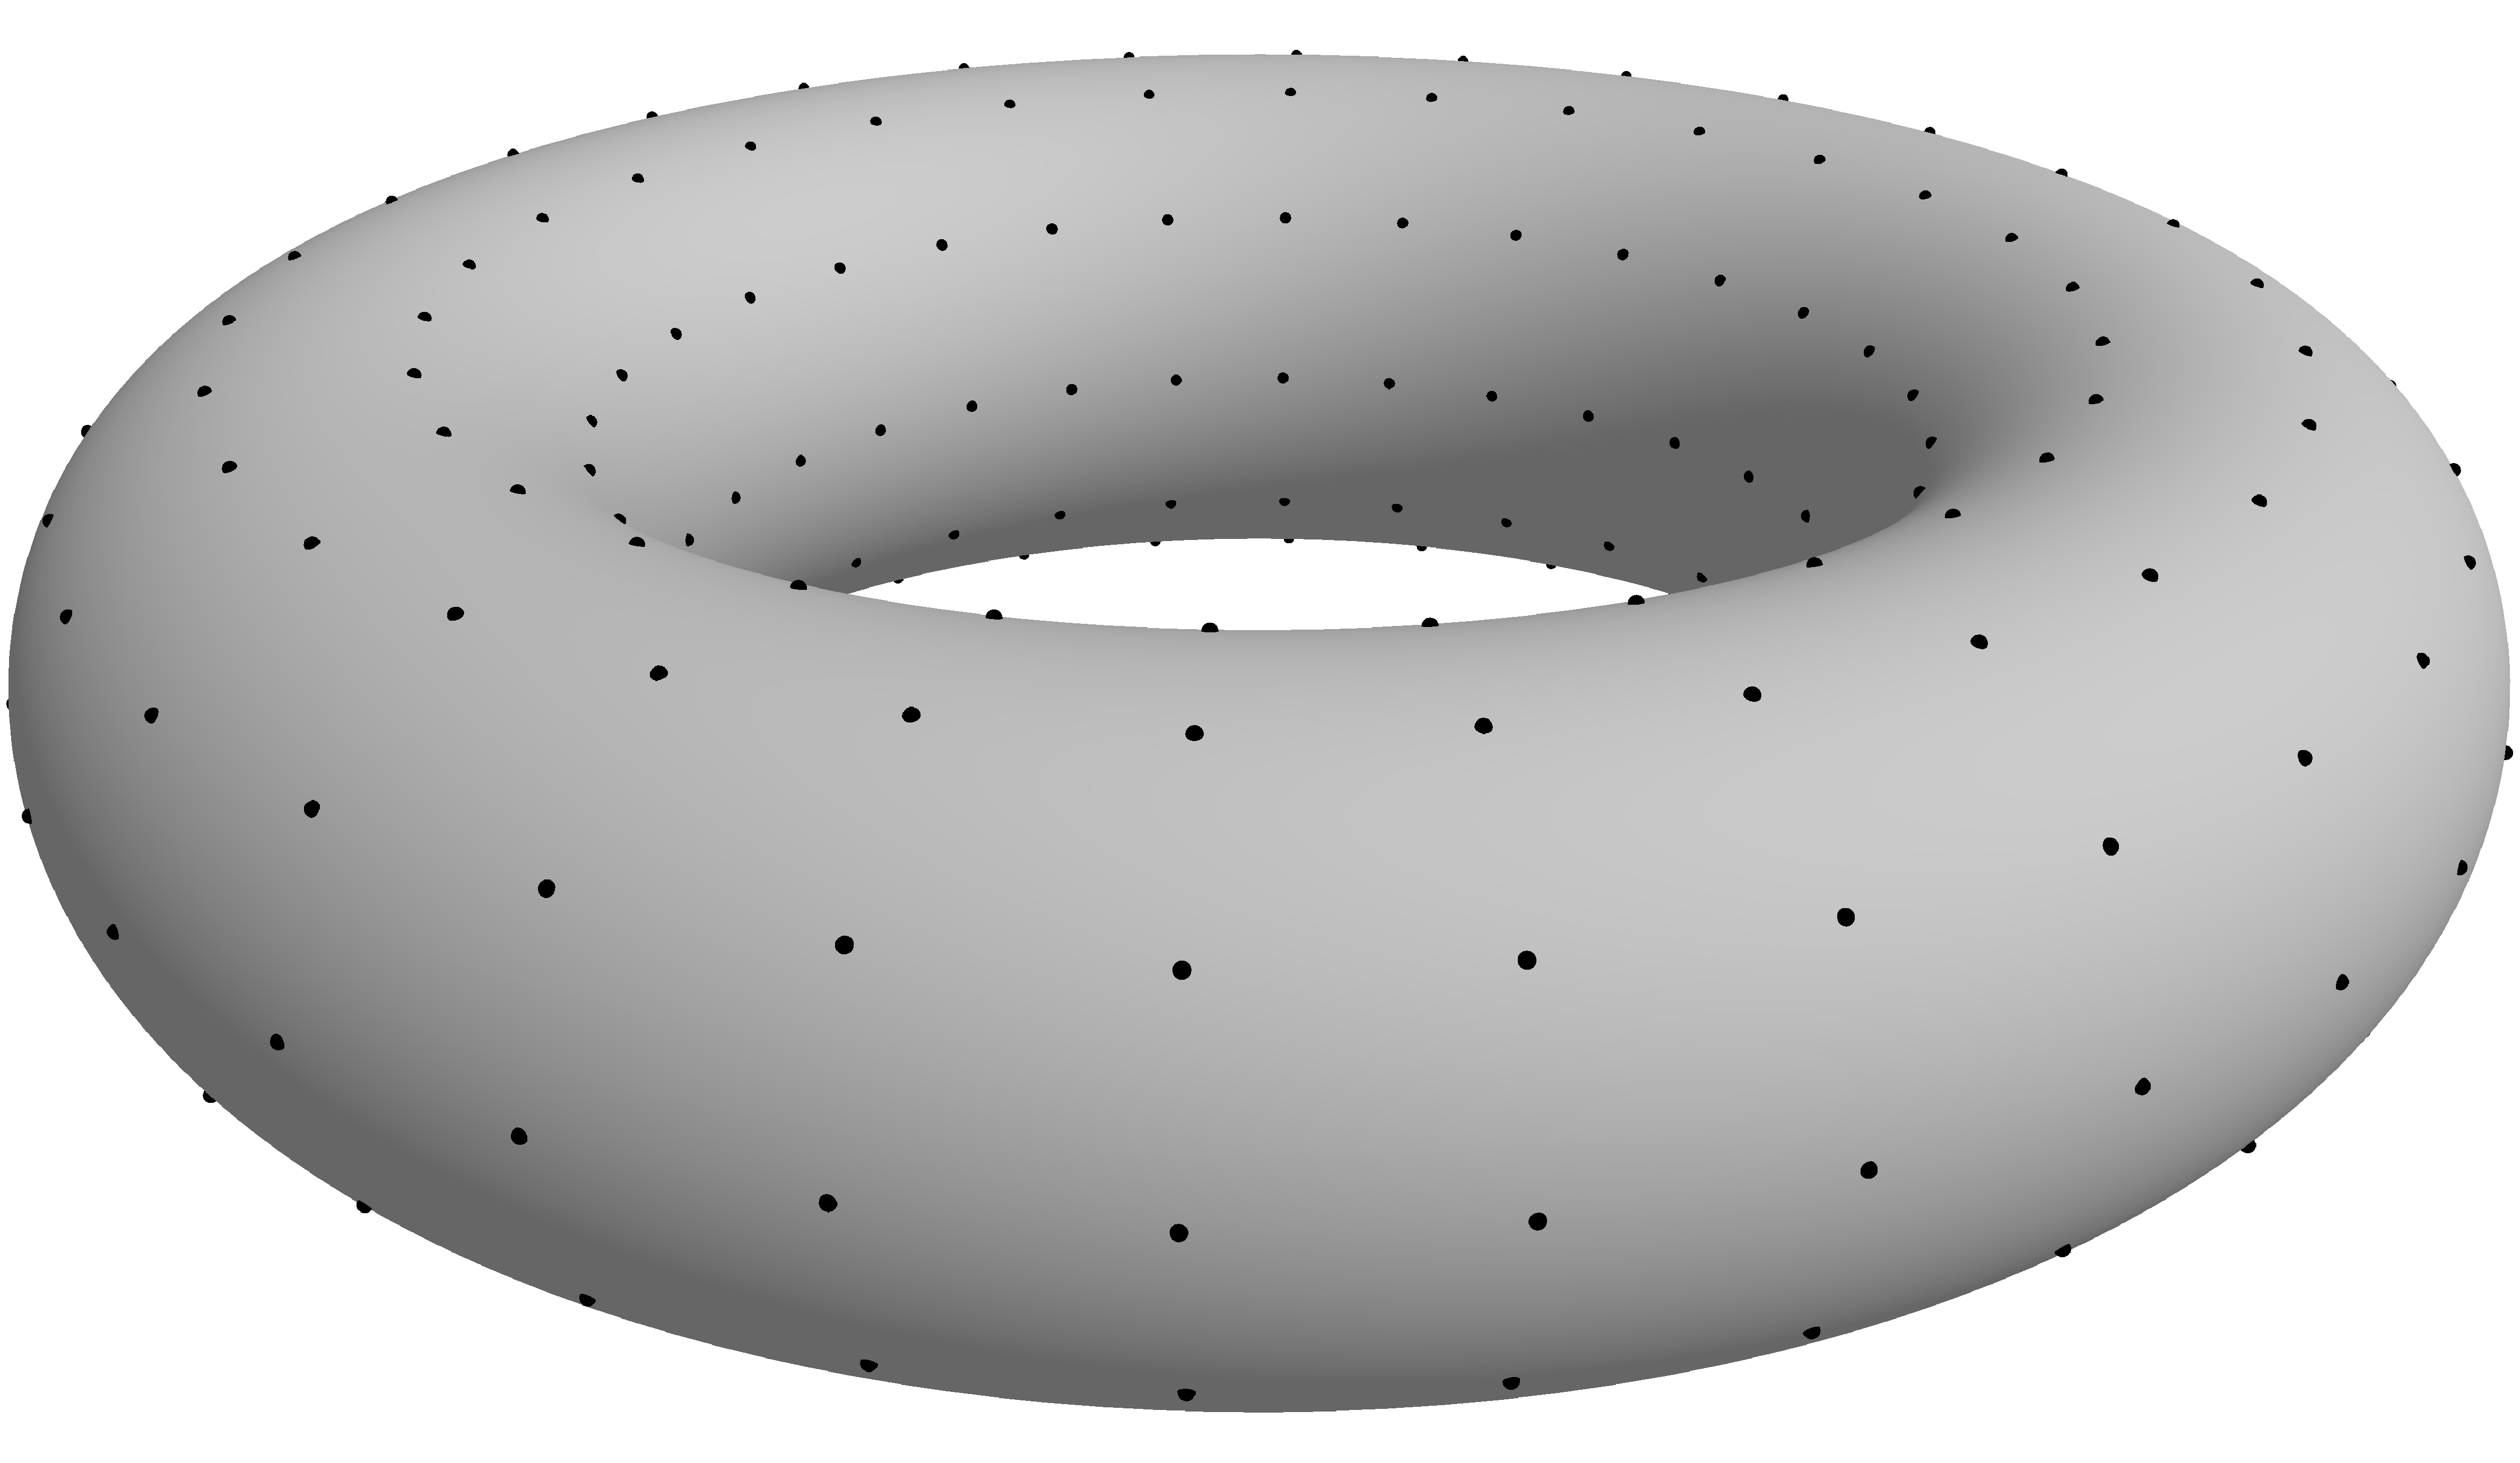
\includegraphics[width=3cm]{torus-with-net}
\end{center}
\par\noindent{}A metric space is \emph{totally bounded} if, for any \(\varepsilon > 0\), the metric space admits a finite open cover by balls of radius \(\varepsilon\); in other words, there is a finite \(\varepsilon\)-net for every \(\varepsilon>0\).
The proof of theorem~\vref{theorem:HB.naive} proves that compact metric spaces are totally bounded.
\begin{problem}{metric.spaces:tot.bdd.discrete}
Which discrete metric spaces are totally bounded?
\end{problem}
\begin{problem}{metric.spaces:tot.bdd.r}
In \(\R{n}\) with the standard discrete metric, are bounded sets totally bounded? the taxi-cab metric? the Euclidean metric? the sup norm metric?
\end{problem}
\begin{theorem}[Heine--Borel\define{Heine--Borel theorem}\define{theorem!Heine--Borel}]\label{theorem:h.b}
In a metric space, a set is compact just when it is complete and totally bounded.
\end{theorem}
\begin{proof}
Compact sets are complete and totally bounded.
Take a complete and totally bounded set.
Take any open cover of the set.
Pick a number \(\varepsilon_1 > 0\).
By total boundedness, we can cover our set in finitely many balls of radius \(\varepsilon\).
Suppose that each of these balls admits a finite cover by our open sets.
Then throw those finitely many covers together to cover the whole set, a finite subcover.
So we can suppose that there is one of these balls, say \(\ball{\varepsilon_1}{x_1}\), which is not covered by any finite number of our open sets.
Cover that ball by finitely many balls of a much smaller radius \(\varepsilon_2\), and conclude by the same reasoning that there is a ball, say \(\ball{\varepsilon_2}{x_2}\), which is not covered by any finite number of our open sets, with \(d\of{x_1,x_2}<\varepsilon_1\).
Inductively, generate a Cauchy sequence \(x_1, x_2, \dots\).
Replace with a subsequence to ensure convergence, say to some point \(x\).
But \(x\) is covered by one of our open sets, so therefore all points close enough to \(x\) are as well.
So one of the balls \(\ball{\varepsilon_j}{x_j}\) lies in that open set, a contradiction.
\end{proof}
A metric space is \emph{locally compact}\define{locally compact!metric space}\define{metric!space!locally compact} if every point lies in the interior of a compact set, and \emph{proper}\define{proper!metric space}\define{metric!space!proper} if every closed ball is compact.
Proper spaces are locally compact.
\begin{problem}{metric.spaces:proper}
Give an example of an improper locally compact metric space.
\end{problem}
\begin{answer}{metric.spaces:proper}
Any infinite set with standard discrete metric: balls of radius 2 are not compact, because the open cover by balls of radius \(1/2\) has no finite subcover, so not all balls are compact.
But the closed balls of radius \(1/2\) are compact, each being just a single point.
\end{answer}
\section{Compactness radius}
The \emph{compactness radius}\define{compactness radius}\define{radius!compactness} of a point \(x \in X\) in a metric space \(X\) is the supremum radius of a compact closed ball around \(x\), zero if there no such ball, infinite if balls of all radii about \(x\) are compact.
\begin{problem}{metric.spaces:radius.cpt.plane}
Find the compactness radius of a point \((x,y) \in X=\R{2}-\left\{(0,0)\right\}\) with metric induced from the Euclidean metric.
\end{problem}
\begin{problem}{metric.spaces:radius.cpt.1}
Prove that if a closed ball lies in a compact closed ball, then it is compact.
\end{problem}
\begin{problem}{metric.spaces:radius.cpt}
Prove that the compactness radius satisfies \(r(y) + d(x,y) \ge r(x)\) for any two points \(x\) and \(y\).
\end{problem}
\begin{answer}{metric.spaces:radius.cpt}
%\begin{center}

\begin{tikzpicture}[scale=.4]
\fill[gray!15] (0,0) circle (1cm);
\fill[gray!25] ({.75*cos(30)},{.75*sin(30)}) circle (.25cm);
\end{tikzpicture}
%\end{center}
\end{answer}
\begin{problem}{metric.spaces:radius.cpt.3}
Prove that the compactness radius is finite at one point just when it is finite at all points.
Prove that the compactness radius is positive everywhere just when the metric is locally compact. Prove that the compactness radius is infinite somewhere, and therefore everywhere, just when the metric is proper.
\end{problem}
\begin{answer}{metric.spaces:radius.cpt.3}
Immediate from \(r(y) + d(x,y) \ge r(x)\): if \(r(x)\) is infinite then so is \(r(y)\).
\end{answer}
\begin{problem}{metric.spaces:radius.cpt.2}
Prove that the compactness radius is continuous if finite.
\end{problem}
\begin{answer}{metric.spaces:radius.cpt.2}
In problem~\vref{problem:metric.spaces:radius.cpt} we saw that \(r(y)+d(x,y) \ge r(x)\), and by symmetry \(r(x)+d(x,y) \ge r(y)\).
Therefore \(d(x,y) \ge |r(x)-r(y)|\), so that if we make \(y \to x\), we find \(r(y) \to r(x)\).
\end{answer}
\begin{problem*}{metric.spaces:radius.cpt.4}
Prove that every connected, locally compact metric space is a countable union of compact sets.
\end{problem*}
\begin{answer}{metric.spaces:radius.cpt.4}
If the compactness radius is somewhere infinite, the space is proper, so its balls of positive integer radius are compact, and it is the union of these.
So assume that the compactness radius is everywhere finite.
By local compactness, the compactness radius is everywhere positive and \(d(x,y)\ge|r(x)-r(y)|\), so the compactness radius is continuous.
Taking any compact set \(K \subset X\), let \(K'\) be the union of all closed balls of radius \(r(x)/2\) about points \(x \in K\).
Any infinite sequence \(x_1,x_2,\dots \in K'\) has each \(x_i\) at distance at most \(r(y_i)/2\) from some \(y_i \in K\).
Take a convergent subsequence of \(y_1,y_2,\dots\), and replace the original sequence with the subsequence, so \(y_1,y_2,\dots \to y\) say.
Then \(d(x_i,y_i)\le r(y_i)/2 \to r(y)/2\).
Far enough down the sequence \(x_1,x_2,\dots\), every \(x_i\) lies in the compact ball of radius \(3r(y)/2\) about \(y\).
Thus \(x_1,x_2,\dots\) has a convergent subsequence.
\end{answer}

\section{Density}
A subset \(A \subset X\) of a metric space is \emph{dense}\define{dense} in another subset \(B\) if the closure of \(A\) contains \(B\), and \emph{everywhere dense}\define{everywhere dense}\define{dense!everywhere} if \(A\) is dense in \(X\).
A metric space is \emph{separable} if it contains a dense sequence of points.
\begin{example}
The rational numbers are dense in the real numbers.
\end{example}
\begin{example}
For each rational number \(q \in \Q{}\), take the set \(U_q \defeq \set{x \in \R{}|x \ne q}\).
So the various \(U_q \subset \R{}\) are dense open sets.
Their intersection 
\[
\bigcap_{q \in \Q{}} U_q \subset \R{}
\]
is precisely the set of irrational numbers, not open, but still dense.
Roughly speaking, if we only pull out a single rational at each step, we still have a lot left over after an infinite sequence of steps.
\end{example}
A set \(A \subset X\) in a metric space is \emph{nowhere dense}\define{dense!nowhere}\define{nowhere dense} if, for any open set \(U \subset X\), \(A \cap U\) is not dense in \(U\).
\begin{example}
The integers are nowhere dense in the real numbers.
\end{example}

\section{The Baire category theorem}
A \emph{meager set} is a subset \(S \subset X\) of a metric space, 
which can somehow be written as
\[
S = C_1 \cup C_2 \cup \dots
\]
as the union of a sequence of nowhere dense closed sets.
\begin{example}
For each rational number \(q \in \Q{}\), take the set \(\set{q} \subset \R{}\).
The various \(\set{q} \subset \R{}\) are nowhere dense closed sets.
Their union, \(\Q{}\), is dense, and not closed, but is still not ``very large'': it has dense complement.
\end{example}
A \emph{comeager}\define{comeager} set is a subset \(A \subset X\) of a metric space, which can somehow be written as
\[
A = U_1 \cap U_2 \cap \dots
\]
as the intersection of a sequence of dense open sets.
\begin{problem}{metric.spaces:comeager}
Prove that a subset of a metric space is meager just when its complement is comeager.
\end{problem}
\begin{theorem}[Baire category theorem]\label{theorem:Baire.category}\define{Baire category theorem}\define{theorem!Baire category}
In any complete metric space, every meager set has dense complement.
In other words, in any complete metric space, every comeager set is dense.
\end{theorem}
\begin{proof}
Take a comeager set
\[
A = U_1 \cap U_2 \cap \dots
\]
Since \(U_1\) is open, it contains a ball.
Since \(U_2\) is open and dense, it contains a ball nested inside the previous ball, and so on.
The Cauchy sequence of centers of the balls \(x_1, x_2, \dots\) converges, say to \(x \in X\).
Since the balls are nested, the point \(x\) is inside all of them.
So the intersection is not empty.

Pick a point \(x \in X\).
Since \(U_1\) is open and dense, it contains balls of radii as small as we like and as close as we like to \(x\).
For any one of these balls, we start the process of the previous paragraph, generating a point of the intersection inside that ball.
Changing the choice of ball, we can make those points approach \(x\).
\end{proof}
\begin{example}
Any countable subset \(S \subset \R{}\) of real numbers has dense complement.
Proof: The complete metric space \(X=\R{}\) contains the nowhere dense closed sets \(\set{x}\) for each point \(x\) of \(X\). 
Apply the Baire category theorem to any sequence of these.
\end{example}
\begin{example}
Take a sequence of polynomial functions \(p_1(x,y), p_2(x,y), \dots\) in two variables \(x,y\), each function nonzero somewhere.
Associate to each polynomial \(p_j(x,y)\) its set of zeroes \(V_j\defeq\set{(x,y)|p_j(x,y)=0}\).
The complete metric space \(X=\R{2}\) contains the nowhere dense closed sets \(V_j\).
By the Baire category theorem, the union
\[
S \defeq V_1 \cup V_2 \cup \dots
\]
has dense complement: you can avoid satisfying \emph{all} of the polynomial equations \(p_j(x,y)=0\) by slight perturbation of any point \((x,y) \in \R{2}\).
\end{example}
\begin{problem}{metric.spaces:Q.metric}
Suppose that we pick a metric on the set \(X \subset \R{}\) of all rational numbers, perhaps not the usual metric.
Suppose that the open sets of this metric are the usual open sets, as from the usual metric.
Prove that \(X\) is not complete.
\end{problem}
\begin{problem}{metric.spaces:no.isolated}
Suppose that \(X\) is a metric space with no isolated points.
Prove that \(X\) is incomplete or uncountable.
\end{problem}
